
\title{Research Summary}
%\date{\today}

\documentclass[12pt]{report}
\usepackage{amsmath,amsxtra,amssymb,latexsym, amscd,amsthm}
\usepackage{url}
\usepackage{color}
\usepackage[mathscr]{eucal}
\usepackage{amsfonts}
\usepackage{graphicx}
\usepackage{fancybox}
\usepackage{multirow}
\usepackage{multicol}
\usepackage{array}
\usepackage[T1]{fontenc}
\usepackage[utf8]{inputenc}
\usepackage[english,vietnamese]{babel}
\usepackage[autostyle]{csquotes}
\usepackage{balance}
\usepackage[nottoc]{tocbibind}
\usepackage{float}
\usepackage{geometry}
\usepackage{lipsum}
\geometry{ a4paper, total={210mm,297mm},  left=20mm, right=20mm,  top=20mm, bottom=20mm }

\newcolumntype{L}[1]{>{\raggedright\let\newline\\\arraybackslash\hspace{0pt}}m{#1}}
\newcolumntype{C}[1]{>{\centering\let\newline\\\arraybackslash\hspace{0pt}}m{#1}}
\newcolumntype{R}[1]{>{\raggedleft\let\newline\\\arraybackslash\hspace{0pt}}m{#1}}
\newcommand\tab[1][1cm]{\hspace*{#1}}
\renewcommand{\bibname}{References}

\begin{document}

\thispagestyle{empty}
\begin{center}

	\vspace*{3cm}
	{\bf \LARGE BÁO CÁO ĐỒ ÁN}\\
	\vspace*{2cm}
	Tên đề tài:\\
	{\bf \Large Open-Set Grounded Text-to-Image Generation}\\
	\vspace{3cm}
	{\Large Trường Đại Học Công Nghệ Thông Tin}\\
	\vspace{5cm}
	%{\Large DOAN DUY}\\
	{\Large Tháng 8/2024}
\end{center}
%\thispagestyle{empty}

\newpage
\vspace*{5cm}
\begin{center}
	{\bf \Large Thông Tin Học Viên}\\
	Tên HV: \tab Mã HV:\\
	Nguyễn Công Danh \tab 230101033\\
	\vspace{5cm}
	{\bf \Large Giảng Viên Hướng Dẫn}\\
	TS. Mai Tiến Dũng
\end{center}

%	\frontmatter
\newpage
%%%%%%%%%%%%%%%%%%%%%%%%%%%%%%%%%%%%%%%%%%%
%+ Acknowledgment
%+ Revised: 17-08-2024
%+ Last revised: 17-08-2024
%%%%%%%%%%%%%%%%%%%%%%%%%%%%%%%%%%%%%%%%%%%
\section*{\centering{Lời cảm ơn}}
%\addcontentsline{toc}{chapter}{Acknowledgements}
Em xin chân thành cảm ơn thầy TS. Mai Tiến Dũng,
người đã tận tình giảng dạy và truyền đạt kiến thức quý báu về môn học Xử lý Ảnh và Thị giác Máy tính.
Sự nhiệt tình, tận tâm của thầy trong việc hướng dẫn
và hỗ trợ em trong suốt quá trình học tập đã giúp em hiểu sâu hơn về các khái niệm,
phương pháp cũng như ứng dụng thực tiễn trong lĩnh vực này.

Nhờ sự chỉ dẫn của thầy,
em đã có thể phát triển được kiến thức và kỹ năng cần thiết
để tự tin hơn trong con đường học tập và nghiên cứu của mình.
Em xin gửi lời cảm ơn chân thành và lòng biết ơn sâu sắc đến thầy.

Kính chúc thầy nhiều sức khỏe và tiếp tục thành công trong sự nghiệp giảng dạy và nghiên cứu.


\begin{flushright}
    Nguyễn Công Danh.
\end{flushright}

%%%%%%%%%%%%%%%%%%%%%%%%%%%%%%%%%%%%%%%%%%%
%+ End of Acknowledgment
%%%%%%%%%%%%%%%%%%%%%%%%%%%%%%%%%%%%%%%%%%%

\tableofcontents
\listoffigures
\listoftables
%\pagenumbering{arabic}
\chapter{Giới thiệu}

\begin{figure}[ht]
	\begin{center}
		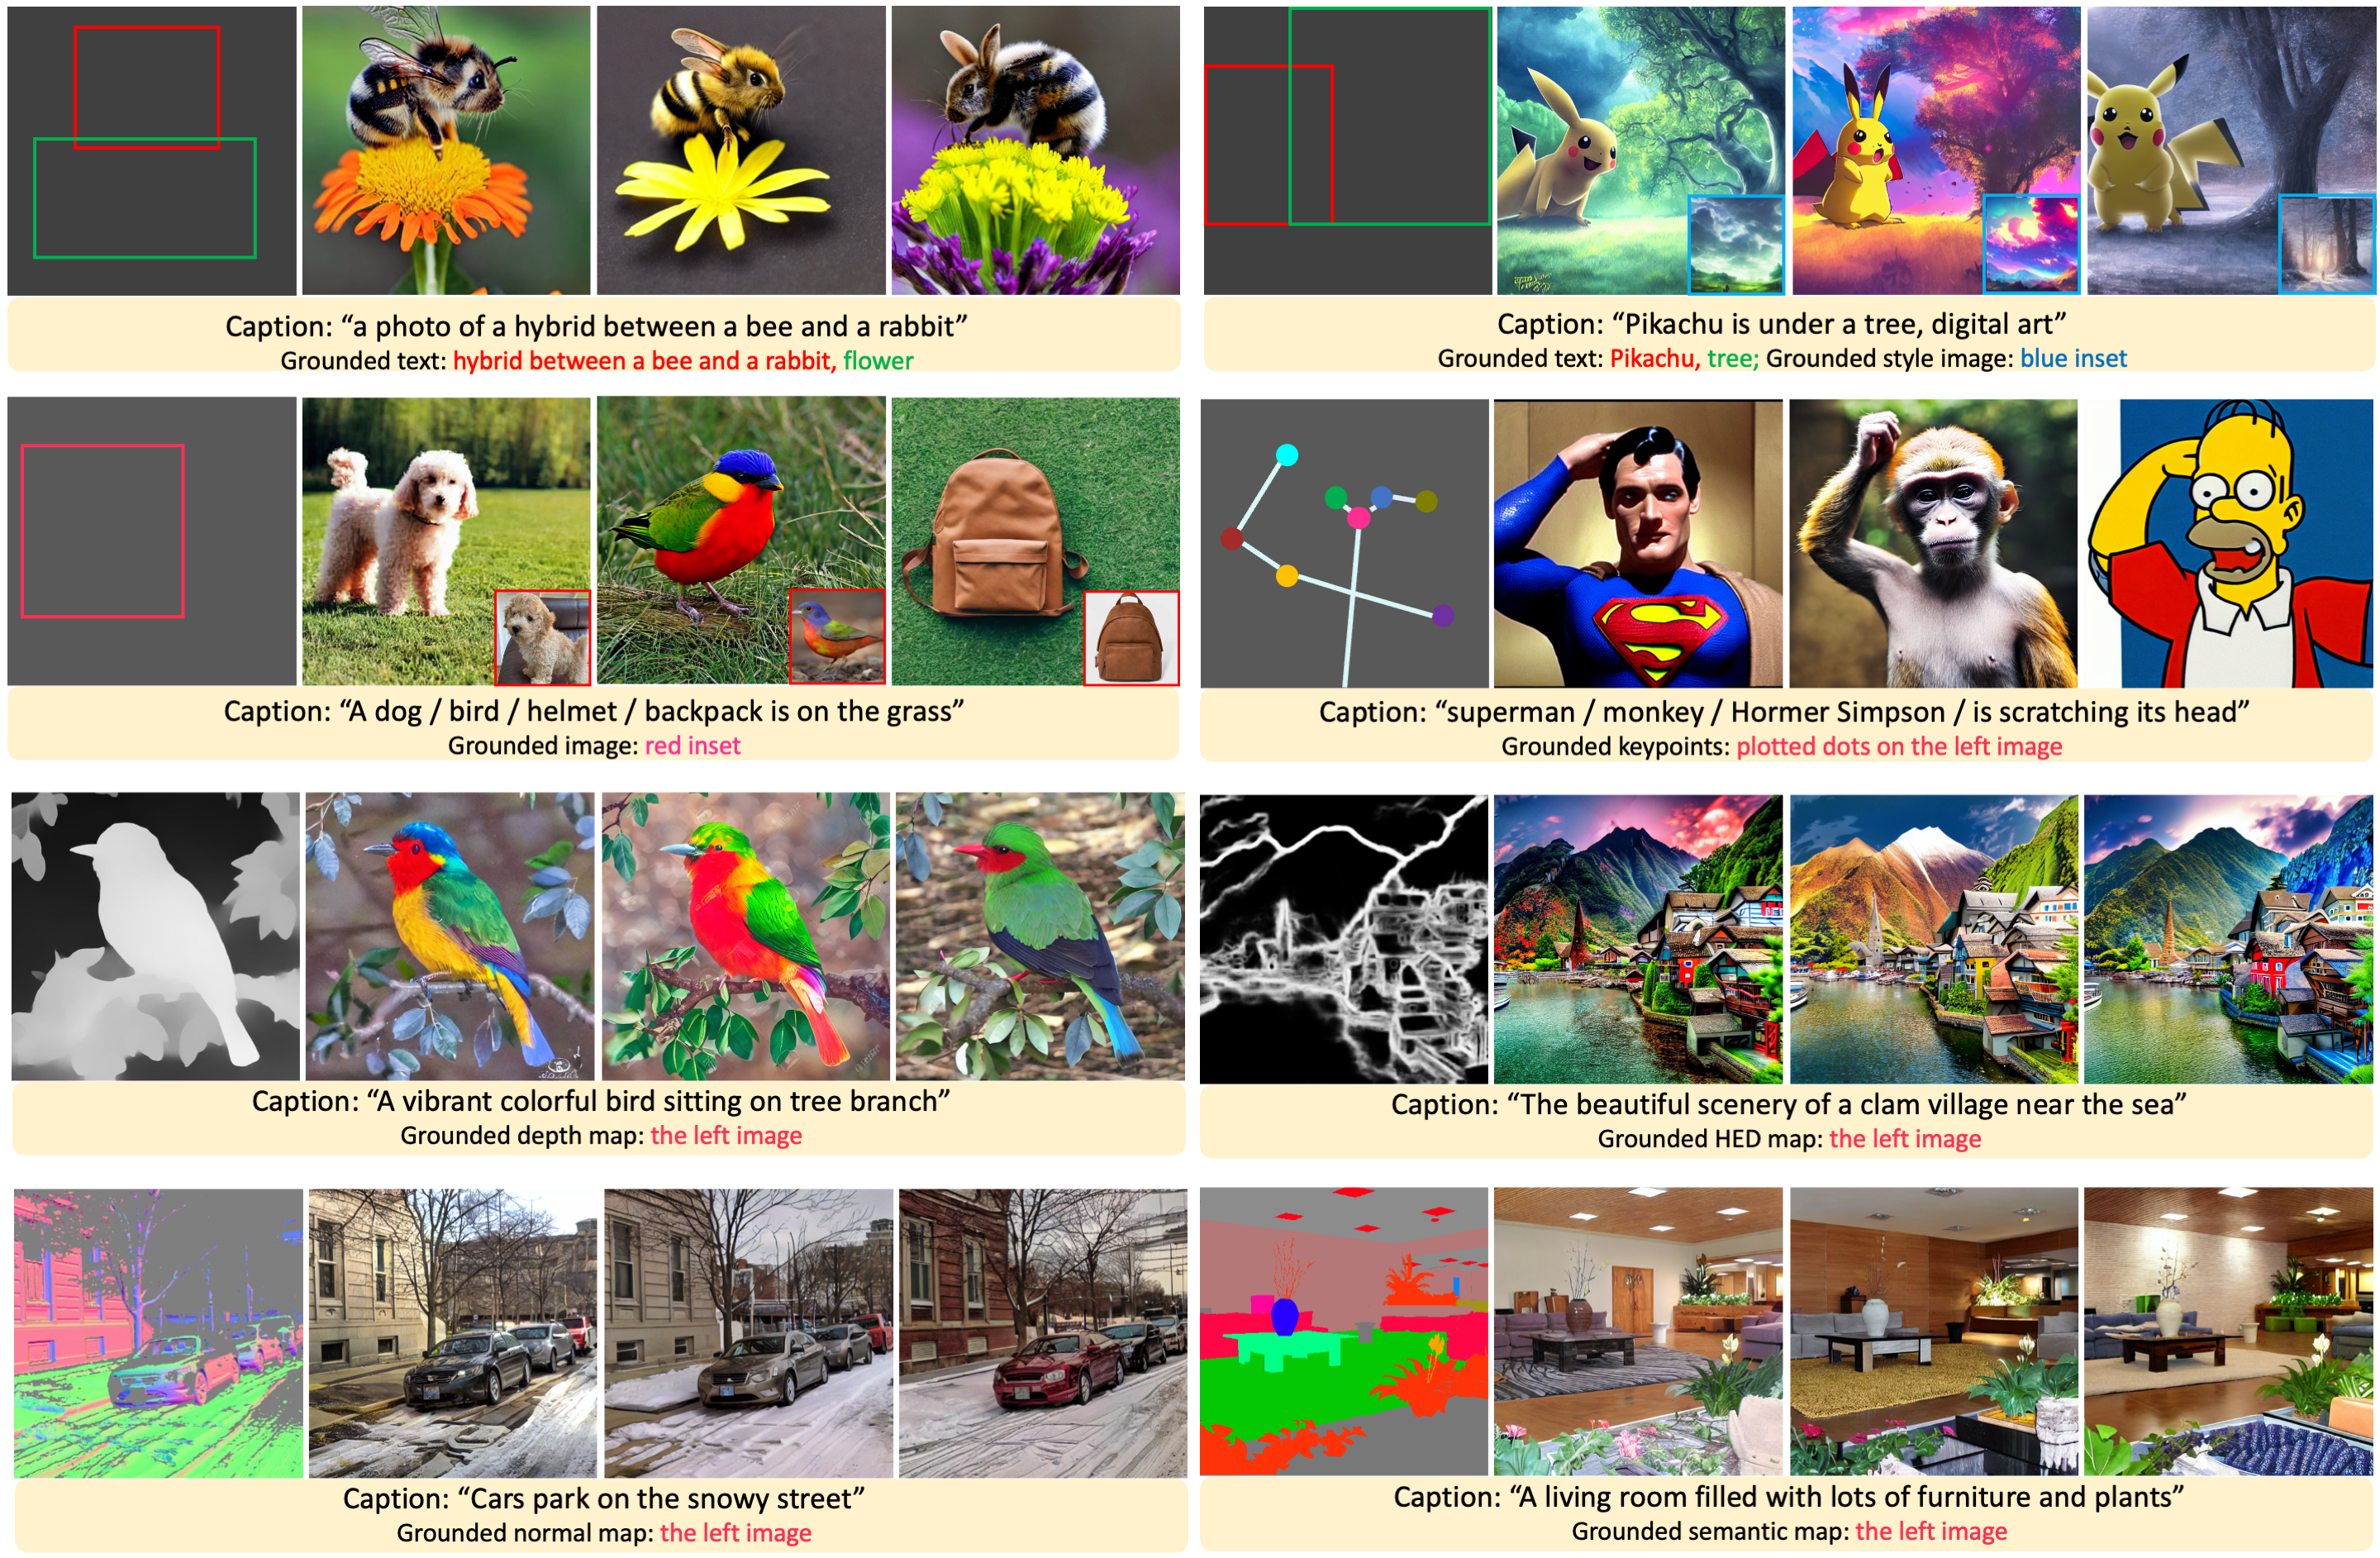
\includegraphics[width=\textwidth]{GligenExamples.png}
		\caption{Những ví dụ về GLIGEN}\label{fig:GligenExamples}
	\end{center}
\end{figure}

\section{Lý do chọn đề tài}
\begin{itemize}
	\item \textbf{Tiên phong trong lĩnh vực nghiên cứu:}
	      Đề tài này liên quan đến một phương pháp mới có tên là GLIGEN,
	      cho phép tạo ra hình ảnh từ văn bản có tính năng kiểm soát cao.
	      Phương pháp này mở rộng khả năng của các mô hình trước đó bằng cách cho phép sử dụng các thông tin đầu vào
	      bổ sung như bounding box, keypoints, canny map, depth map, normal map, hed map và semantic map.

	\item \textbf{Đóng góp lớn cho cộng đồng học thuật:}
	      GLIGEN đã được đánh giá và chứng minh có khả năng vượt trội so với các mô hình trước đây
	      trong việc tạo hình ảnh dựa trên văn bản ở các nhiệm vụ mới và đa dạng,
	      điều này giúp đóng góp lớn cho cộng đồng nghiên cứu trong việc nâng cao chất lượng
	      và độ chính xác của các hệ thống tạo hình ảnh.

	\item \textbf{Tính ứng dụng cao:}
	      Phương pháp GLIGEN không chỉ cải thiện về mặt lý thuyết
	      mà còn có tiềm năng ứng dụng rộng rãi trong nhiều lĩnh vực như thiết kế đồ họa
	      và tạo nội dung số.
\end{itemize}

\section{Phát biểu bài toán}

Bài toán trong bài báo này được phát biểu như sau:
\begin{itemize}
	\item Input: Đầu vào bao gồm một chú thích văn bản (caption)
	      và các thông tin định vị (grounding information) như hộp giới hạn (bounding boxes),
	      điểm mốc (keypoints), có thể được mô tả bằng văn bản hoặc hình ảnh tham chiếu.
	\item Output: Đầu ra là hình ảnh được sinh ra dựa trên chú thích văn bản
	      và các thông tin định vị, đảm bảo rằng hình ảnh này thể hiện chính xác các yếu tố
	      và vị trí của chúng theo đầu vào đã cung cấp.
\end{itemize}

\section{Kết quả mong đợi}
Kết quả mong đợi khi thực hiện đề tài này là tìm hiểu một phương pháp mới
có khả năng tạo ra hình ảnh từ văn bản và thông tin định vị với độ chính xác cao.

\section{Phạm vi/Giới hạn}
Khi thực hiện đề tài này, em sẽ tập trung vào việc tìm hiểu phương pháp,
cách cài đặt và sử dụng lại mô hình có sẵn.
Không đi sâu vào việc nghiên cứu và phát triển mô hình mới.

\chapter{Phương pháp}

Phương pháp được đề xuất trong bài báo nhằm mục đích mở rộng khả năng của các mô hình khuếch tán
(diffusion models) trong việc sinh ra hình ảnh từ văn bản,
bằng cách tích hợp thêm thông tin định vị (grounding information)
như hộp giới hạn (bounding boxes), điểm mốc (keypoints).
Dưới đây là mô tả chi tiết về phương pháp giải quyết này:

\section{Kiến trúc tổng quan của GLIGEN}
GLIGEN được xây dựng dựa trên các mô hình khuếch tán văn bản-đến-hình ảnh đã được huấn luyện trước đó,
như GLIDE hoặc Stable Diffusion.
Phương pháp này thêm vào một mô-đun điều khiển tổng quát (generic gating module)
để tích hợp thông tin định vị vào quá trình sinh hình ảnh. Thành phần chính của GLIGEN bao gồm:
\begin{itemize}
	\item Mô hình khuếch tán cơ bản: Đây là mô hình đã được huấn luyện trước để sinh hình ảnh từ văn bản.
	\item Mô-đun điều khiển (Gating Module):
	      Mô-đun này chịu trách nhiệm kết hợp thông tin định vị với đặc trưng (features)
	      của mô hình khuếch tán thông qua một cơ chế điều khiển linh hoạt.
	\item Bộ mã hóa định vị (Grounding Encoder): Chuyển đổi thông tin định vị
	      (như hộp giới hạn, điểm mốc) thành các biểu diễn số học phù hợp để sử dụng trong mô hình.
\end{itemize}

\section{Cơ chế tích hợp thông tin định vị}
GLIGEN sử dụng một cơ chế điều khiển dựa trên cổng điều khiển (gates)
để tích hợp thông tin định vị vào các lớp của mô hình khuếch tán:
\begin{itemize}
	\item Tích hợp thông tin định vị:
	      Thông tin định vị được mã hóa và sau đó được kết hợp với đặc trưng của mô hình
	      khuếch tán thông qua các cổng điều khiển.
	      Cơ chế này cho phép mô hình linh hoạt điều chỉnh mức độ ảnh hưởng của thông tin định vị
	      tại các vị trí khác nhau trong quá trình sinh ảnh.
	\item Học hỏi linh hoạt: Thông qua việc sử dụng cổng điều khiển,
	      mô hình có thể học cách cân bằng giữa thông tin từ văn bản và thông tin định vị,
	      đảm bảo rằng hình ảnh được sinh ra vừa phản ánh đúng mô tả văn bản,
	      vừa tuân thủ các ràng buộc về vị trí và cấu trúc từ thông tin định vị.
\end{itemize}

\begin{figure}[ht]
	\begin{center}
		\includegraphics[width=0.5\textwidth]{GatedSelfAttention.png}
		\caption{Gated Self-Attention được dùng để kết hợp các thông tin định vị mới}\label{fig:GatedSelfAttention}
	\end{center}
\end{figure}

\section{Quá trình huấn luyện}
GLIGEN được huấn luyện thông qua hai giai đoạn chính:
\begin{itemize}
	\item Huấn luyện tiền huấn luyện (Pre-training):
	      Mô hình được huấn luyện trên một tập dữ liệu lớn bao gồm các cặp văn bản-hình ảnh
	      với thông tin định vị tương ứng.
	      Quá trình này giúp mô hình học được cách kết hợp hiệu quả giữa văn bản
	      và thông tin định vị để sinh ra hình ảnh phù hợp.
	\item Huấn luyện tinh chỉnh (Fine-tuning):
	      Sau khi tiền huấn luyện, mô hình được tinh chỉnh trên các nhiệm vụ cụ thể
	      hoặc các bộ dữ liệu đặc thù để cải thiện hiệu suất và khả năng tổng quát hóa.
\end{itemize}

\section{Ưu điểm của phương pháp}
Phương pháp GLIGEN có một số ưu điểm so với các phương pháp trước đây:
\begin{itemize}
	\item Khả năng điều khiển cao:
	      GLIGEN cho phép người dùng kiểm soát chi tiết về vị trí,
	      kích thước và bố cục của các đối tượng trong hình ảnh thông qua thông tin định vị.
	\item Tổng quát hóa tốt: Mô hình có khả năng tổng quát hóa
	      đến các đối tượng và cấu hình mới không xuất hiện trong dữ liệu huấn luyện,
	      nhờ vào cơ chế điều khiển linh hoạt.
	\item Tích hợp dễ dàng: Phương pháp này có thể được tích hợp vào các mô hình khuếch tán
	      đã được huấn luyện trước mà không cần thay đổi nhiều về kiến trúc,
	      giúp tiết kiệm thời gian và tài nguyên.
\end{itemize}

\section{Kết quả thực nghiệm}
Thực nghiệm trên các bộ dữ liệu như COCO và Visual Genome cho thấy
GLIGEN vượt trội hơn các phương pháp trước đây về khả năng sinh hình ảnh chất lượng cao
và tuân thủ chính xác các ràng buộc định vị.
\begin{figure}[ht]
	\begin{center}
		\includegraphics[width=0.5\textwidth]{COCO2014Comparision.png}
		\caption{Đánh giá chất lượng hình ảnh và sự phù hợp với bố cục
			trên COCO2014 val-set.}\label{fig:COCO2014Comparision}
	\end{center}
\end{figure}

\chapter{Đánh giá và nhận xét}
\section{Ưu điểm}

\begin{itemize}
	\item Phương pháp GLIGEN mở rộng khả năng của các mô hình khuếch tán văn bản-đến-hình ảnh
	      bằng cách tích hợp thông tin định vị, giúp cải thiện chất lượng và độ chính xác của hình ảnh sinh ra.
	\item Mô hình này cho phép kiểm soát chi tiết về vị trí, kích thước và bố cục của các đối tượng trong hình ảnh,
	      giúp tạo ra hình ảnh phản ánh chính xác mô tả văn bản.
	\item GLIGEN có khả năng tổng quát hóa tốt đến các đối tượng và cấu hình mới không xuất hiện trong dữ liệu huấn luyện,
	      nhờ vào cơ chế điều khiển linh hoạt.
	\item Phương pháp này có thể được tích hợp vào các mô hình khuếch tán đã được huấn luyện trước mà không cần thay đổi nhiều về kiến trúc,
	      giúp tiết kiệm thời gian và tài nguyên.
\end{itemize}

\section{Nhược điểm}

\begin{itemize}
	\item Mặc dù GLIGEN đã đạt được kết quả tốt trên các bộ dữ liệu thử nghiệm,
	      nhưng cần thêm nhiều thử nghiệm và đánh giá trên các bộ dữ liệu đa dạng để chứng minh tính tổng quát và hiệu quả của phương pháp.
	\item Phương pháp này cần một lượng dữ liệu huấn luyện lớn để đạt được hiệu suất tốt,
	      điều này có thể là một hạn chế đối với các ứng dụng thực tế.
\end{itemize}
\newpage
\begin{thebibliography}{1}
	\bibitem{ref1}
	Li, Y., Liu, H., Wu, Q., Mu, F., Yang, J., Gao, J., Li, C., \& Lee, Y. J. (2023). GLIGEN: Open-Set Grounded Text-to-Image Generation. In Proceedings of the IEEE/CVF Conference on Computer Vision and Pattern Recognition (CVPR) (pp. 22511-22521).
\end{thebibliography}
\end{document}